\documentclass[unicode,11pt,a4paper,oneside,numbers=endperiod,openany]{scrartcl}

\usepackage{ifthen}
\usepackage[utf8]{inputenc}
\usepackage{graphics}
\usepackage{graphicx}
\usepackage{hyperref}

\pagestyle{plain}
\voffset -5mm
\oddsidemargin  0mm
\evensidemargin -11mm
\marginparwidth 2cm
\marginparsep 0pt
\topmargin 0mm
\headheight 0pt
\headsep 0pt
\topskip 0pt        
\textheight 255mm
\textwidth 165mm

\newcommand{\duedate} {}
\newcommand{\setduedate}[1]{%
\renewcommand\duedate {See iCorsi for due date}}
\newcommand\isassignment {false}
\newcommand{\setassignment}{\renewcommand\isassignment {true}}
\newcommand{\ifassignment}[1]{\ifthenelse{\boolean{\isassignment}}{#1}{}}
\newcommand{\ifnotassignment}[1]{\ifthenelse{\boolean{\isassignment}}{}{#1}}

\newcommand{\assignmentpolicy}{
\begin{table}[h]
\begin{center}
\scalebox{0.8} {%
\begin{tabular}{|p{0.02cm}p{16cm}|}
\hline
&\\
\multicolumn{2}{|c|}{\Large\textbf{HPC Lab ---  Submission Instructions}}\\
\multicolumn{2}{|c|}{\large\textbf{(Please, notice that following instructions are mandatory: }}\\
\multicolumn{2}{|c|}{\large\textbf{submissions that don't comply with, won't be considered)}}\\
&\\
\textbullet & Assignments must be submitted to \href{https://www.icorsi.ch}{iCorsi} (i.e. in electronic format).\\
\textbullet & Provide sources (e.g. C/C++ files, Matlab). 
If you are using libraries, please add them in the file. Sources must be organized in directories called:\\
\multicolumn{2}{|c|}{\textit{Project\_number\_lastname\_firstname}}\\
& and  the  file must be called:\\
\multicolumn{2}{|c|}{\textit{project\_number\_lastname\_firstname.zip}}\\
\multicolumn{2}{|c|}{\textit{project\_number\_lastname\_firstname.pdf}}\\
\textbullet &  The TAs will grade your project by reviewing your project write-up, and looking at the implementation 
                 you attempted, and benchmarking your code's performance.\\

\textbullet & You are allowed to discuss all questions with anyone you like; however: (i) your submission must list anyone you discussed problems with and (ii) you must write up your submission independently.\\
\hline
\end{tabular}
}
\end{center}
\end{table}
}
\newcommand{\punkte}[1]{\hspace{1ex}\emph{\mdseries\hfill(#1~\ifcase#1{Points}\or{Points}\else{Points}\fi)}}


\newcommand\serieheader[6]{
\thispagestyle{empty}%
\begin{flushleft}

\includegraphics[width=0.4\textwidth]{usi_inf.png}
\end{flushleft}
  \noindent%
  {\large\ignorespaces{\textbf{#1}}\hspace{\fill}\ignorespaces{ \textbf{#2}}}\\ \\%
  {\large\ignorespaces #3 \hspace{\fill}\ignorespaces #4}\\
  \noindent%
  \bigskip
  \hrule\par\bigskip\noindent%
  \bigskip {\ignorespaces {\Large{\textbf{#5}}}
  \hspace{\fill}\ignorespaces \large \ifthenelse{\boolean{\isassignment}}{\duedate}{#6}}
  \hrule\par\bigskip\noindent%  \linebreak
 }

\makeatletter
\def\enumerateMod{\ifnum \@enumdepth >3 \@toodeep\else
      \advance\@enumdepth \@ne
      \edef\@enumctr{enum\romannumeral\the\@enumdepth}\list
      {\csname label\@enumctr\endcsname}{\usecounter
        {\@enumctr}%%%? the following differs from "enumerate"
	\topsep0pt%
	\partopsep0pt%
	\itemsep0pt%
	\def\makelabel##1{\hss\llap{##1}}}\fi}
\let\endenumerateMod =\endlist
\makeatother




\usepackage{textcomp}





% Provide improved math macros (\text, etc.) used in the report
\usepackage{amsmath}
\usepackage{amssymb}
\begin{document}


\setassignment

\serieheader{High-Performance Computing Lab}{Institute of Computing}{Student: FULL NAME}{Discussed with: FULL NAME}{Solution for Project 2}{}
\newline

\assignmentpolicy
This project will introduce you to parallel programming using OpenMP. 

\section{Parallel reduction operations using OpenMP \punkte{20}}

\subsection{Dot Product}
\subsection*{1 Parallel Implementations}

Two parallel implementations of the dot product were developed using OpenMP.

\begin{itemize}
    \item \textbf{Reduction Clause:} This method uses \texttt{\#pragma omp parallel for reduction(+:alpha)} to safely accumulate partial results from each thread. It is efficient and minimizes synchronization overhead.
    
    \item \textbf{Critical Directive:} This method uses \texttt{\#pragma omp critical} to serialize access to the shared accumulation variable, ensuring correctness but introducing significant performance penalties due to thread contention.
\end{itemize}

Correctness of both implementations was verified against the serial baseline.

\subsection*{2 Strong Scaling Analysis}

Strong scaling tests were conducted on the Rosa cluster for both parallel versions using thread counts $t = 1, 2, 4, 8, 16, 20$ and vector sizes $N = 10^5, 10^6, 10^7, 10^8, 10^9$.

\subsection*{Reduction Method}

\begin{figure}[h]
    \centering
    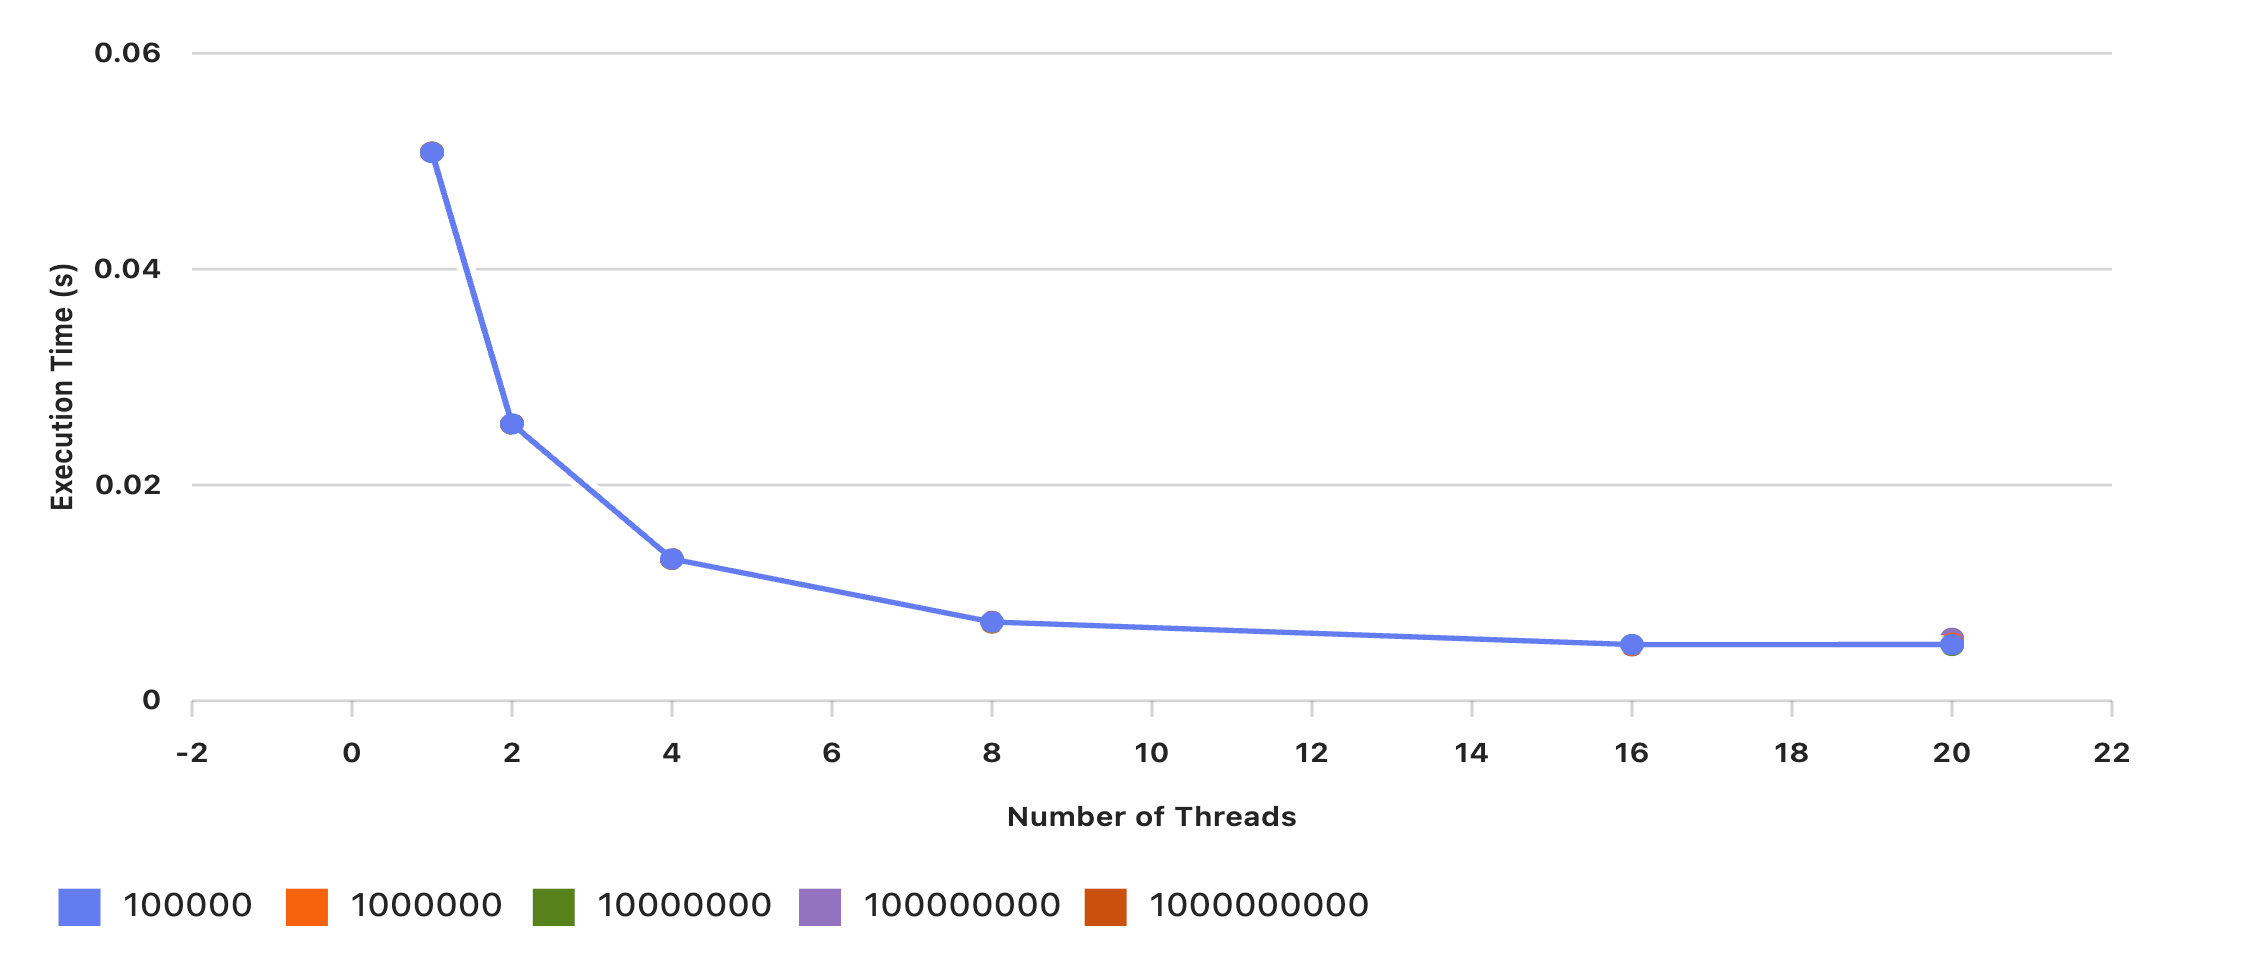
\includegraphics[width=0.8\textwidth]{./figures/Figure 1: Strong Scaling - Reduction Method.png}
    \caption{Strong scaling performance using the reduction method.}
\end{figure}

The reduction method demonstrates consistent improvement in execution time as the number of threads increases. For larger vector sizes, scaling is nearly ideal up to 8 threads, with diminishing returns beyond that point due to hardware limitations and overhead.

\subsection*{Critical Method}

\begin{figure}[h]
    \centering
    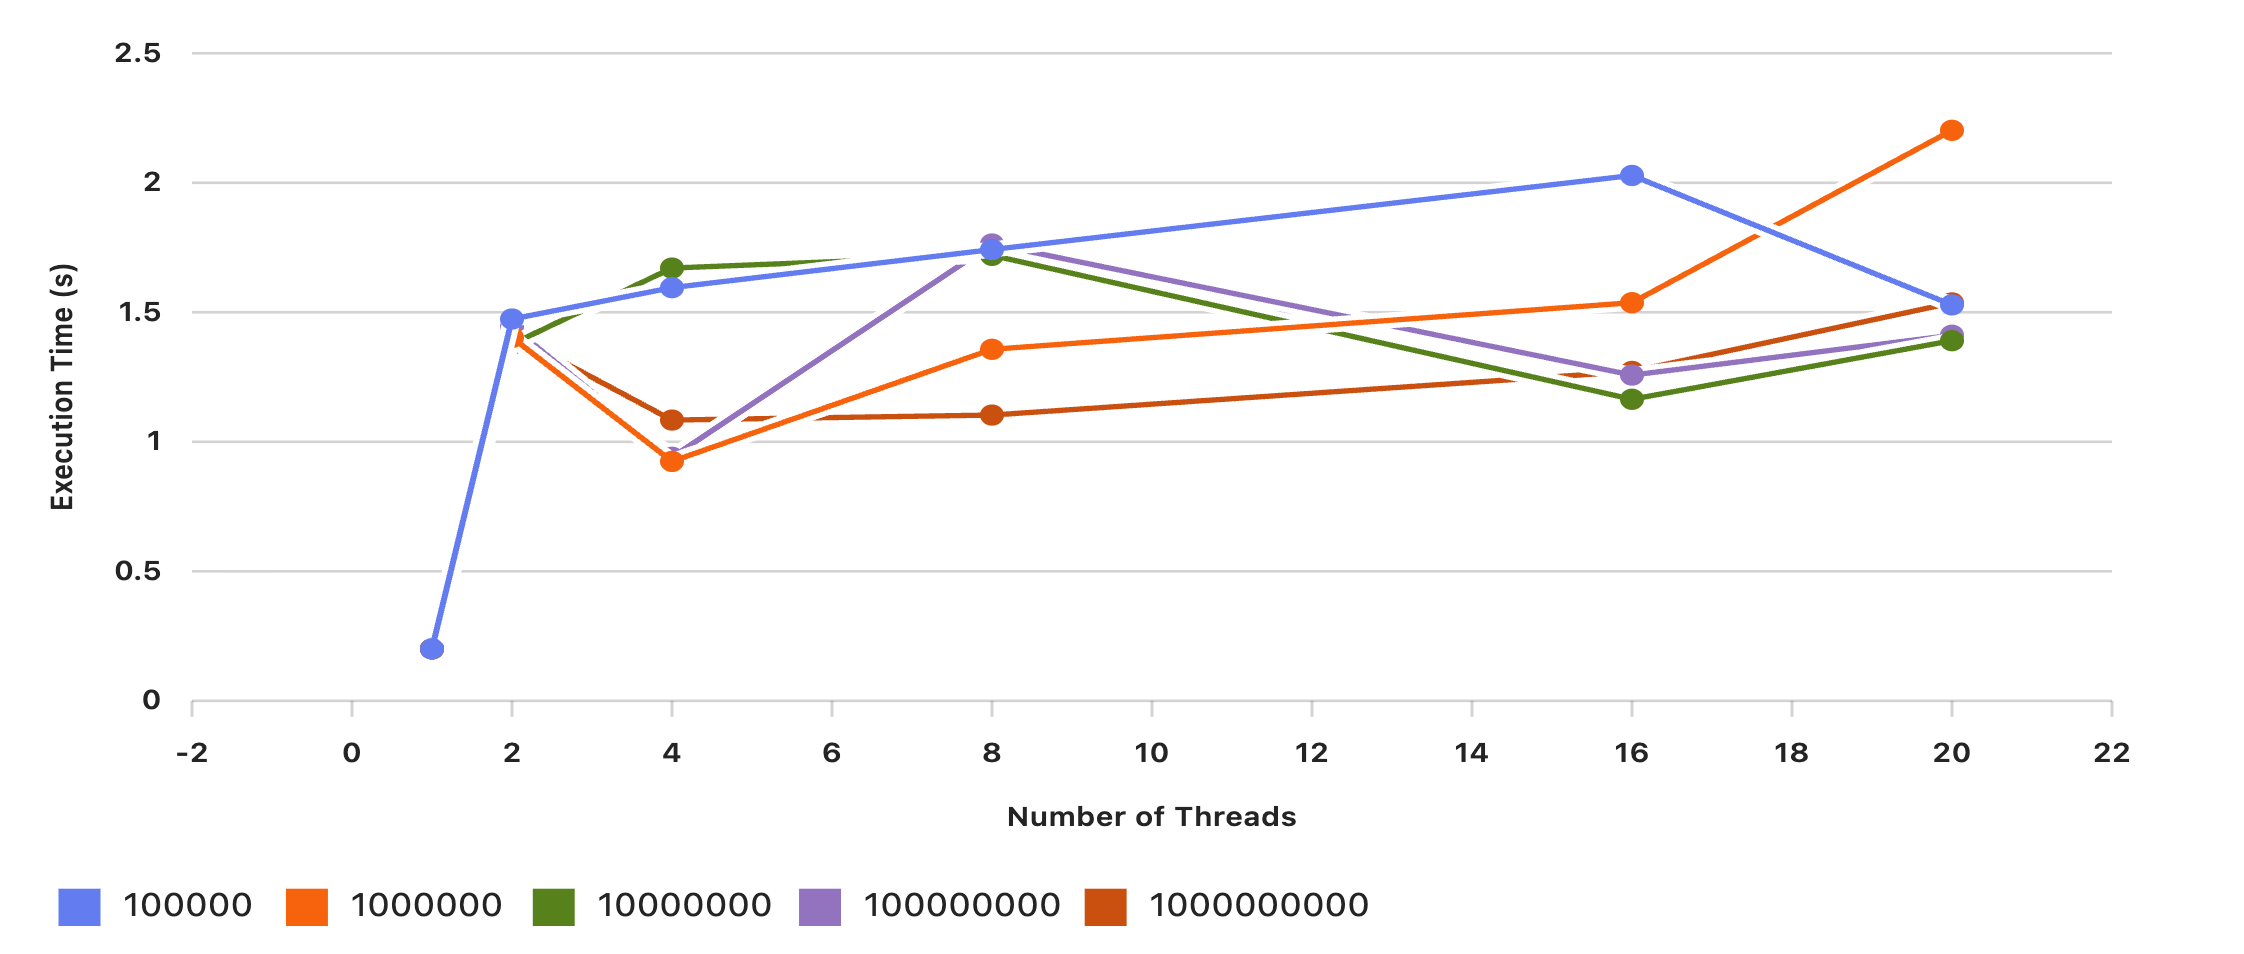
\includegraphics[width=0.8\textwidth]{./figures/Figure 2: Strong Scaling - Critical Method.png}
    \caption{Strong scaling performance using the critical method.}
\end{figure}

The critical method exhibits poor scalability. Execution time increases with additional threads due to contention at the critical section, particularly for small vector sizes. For larger $N$, performance stabilizes but remains significantly inferior to the reduction method.

\newpage
\subsection*{3 Parallel Efficiency Analysis}

Parallel efficiency was computed as:
\[
\text{Efficiency} = \frac{\text{Speedup}}{\text{Number of Threads}}, \quad \text{Speedup} = \frac{\text{Serial Time}}{\text{Parallel Time}}
\]

\subsection*{Reduction Method}

\begin{figure}[h]
    \centering
    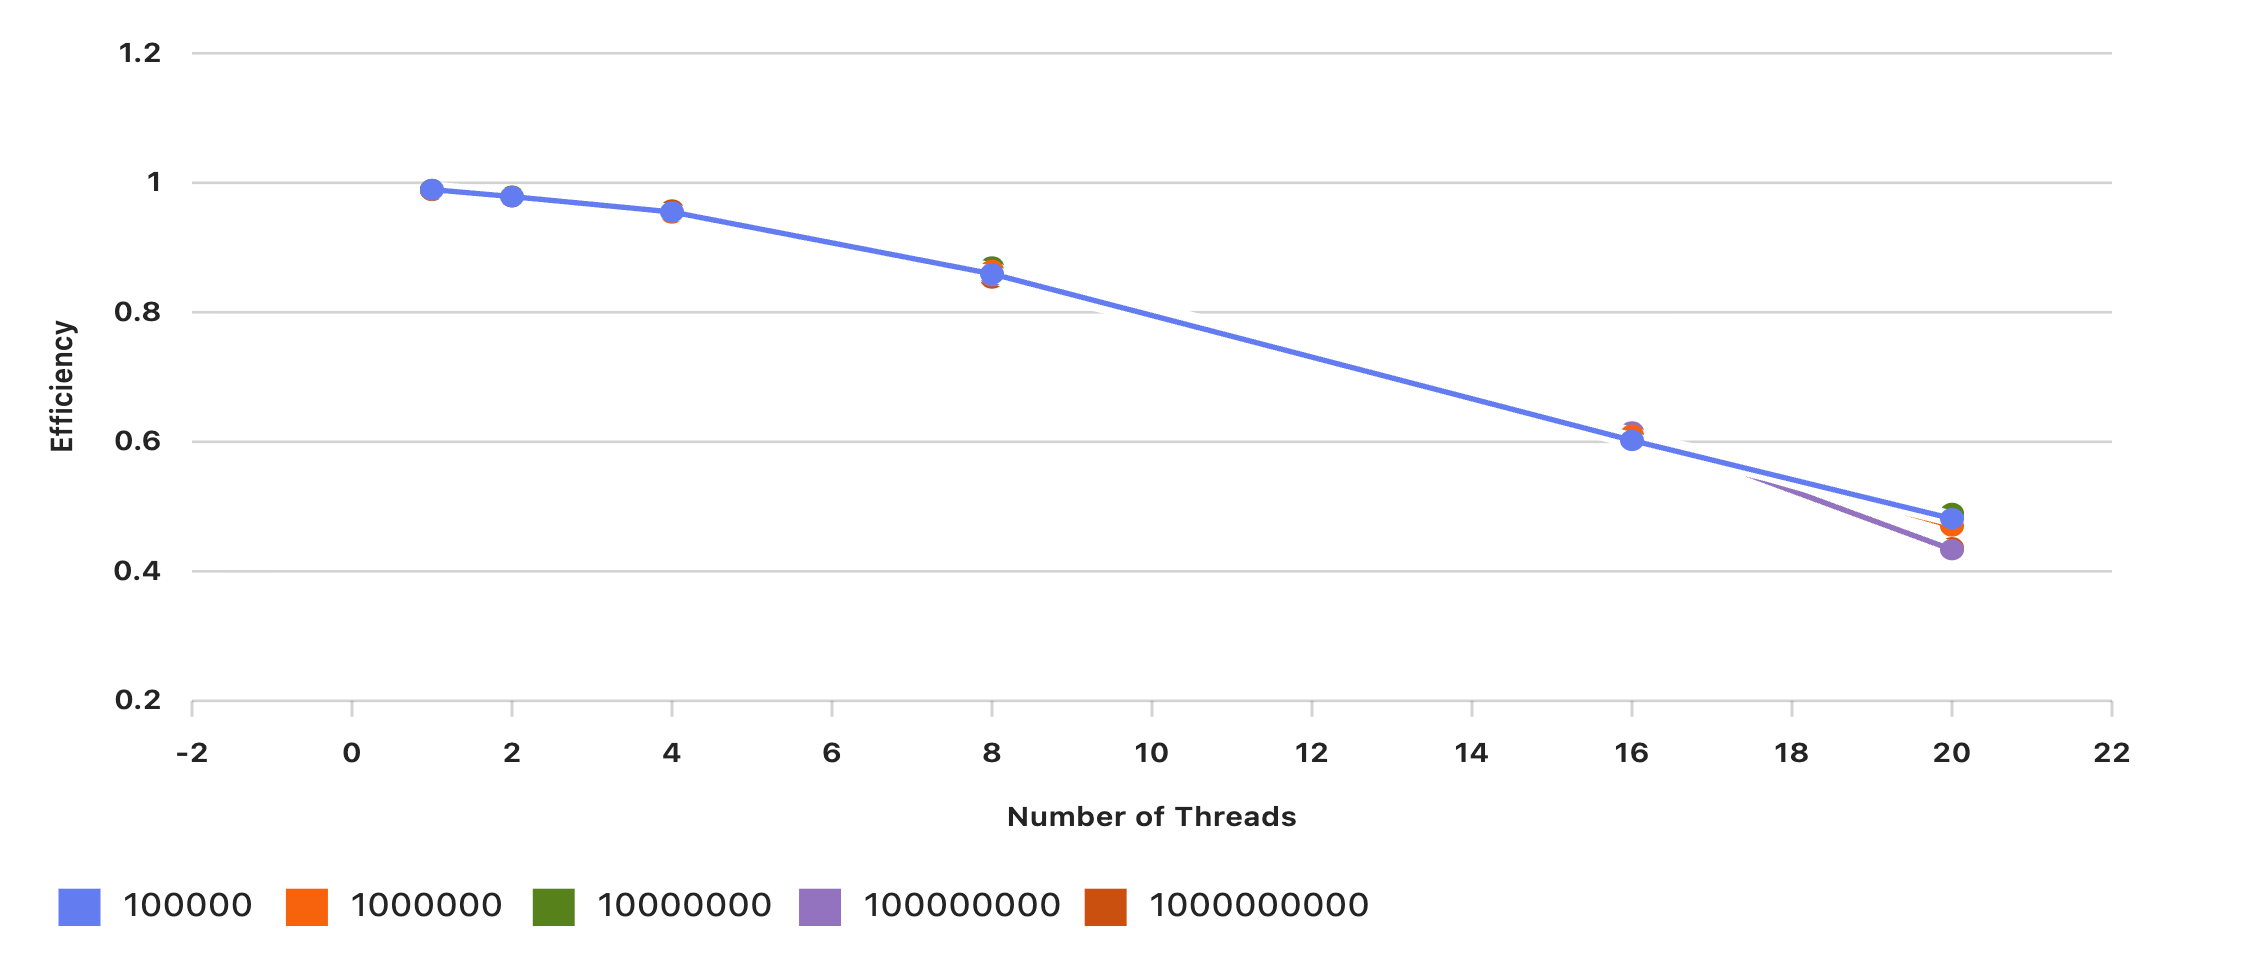
\includegraphics[width=0.8\textwidth]{./figures/Figure 3: Parallel Efficiency - Reduction Method.png}
    \caption{Parallel efficiency using the reduction method.}
\end{figure}

Efficiency remains high for small thread counts and large vector sizes. For $N \geq 10^7$, efficiency exceeds 60\% even at 20 threads, indicating effective utilization of parallel resources.
\subsection*{Critical Method}

\begin{figure}[h]
    \centering
    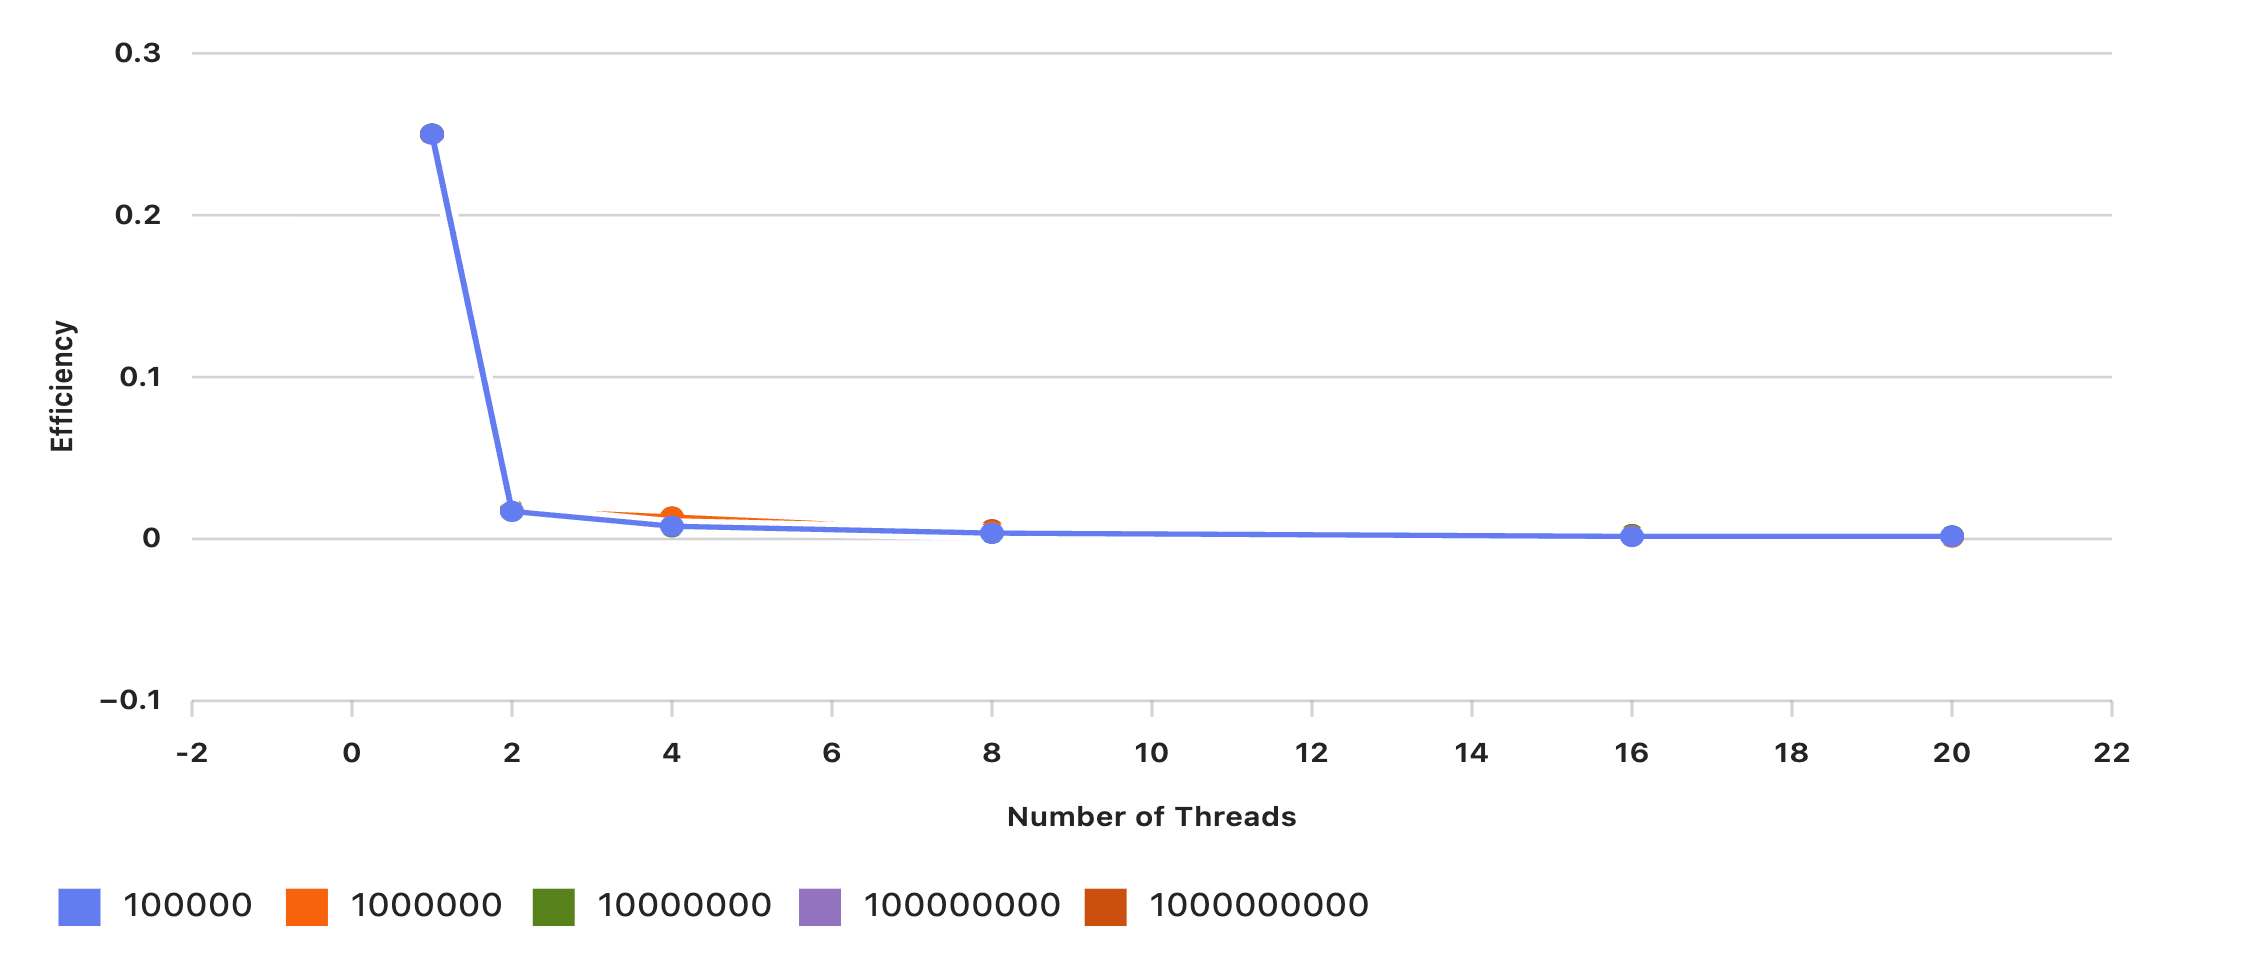
\includegraphics[width=0.8\textwidth]{./figures/Figure 4: Parallel Efficiency - Critical Method.png}
    \caption{Parallel efficiency using the critical method.}
\end{figure}

Efficiency declines sharply with increasing thread counts, particularly for small $N$. Even for $N = 10^9$, efficiency remains low due to synchronization overhead. This behavior is consistent across all vector sizes, confirming that the synchronization cost outweighs the benefits of parallelism.

\newpage
\section*{Discussion}

\subsection*{OpenMP Overhead}

The critical directive introduces significant overhead due to serialized access to the shared variable. In contrast, the reduction clause avoids this issue by efficiently combining partial results.

\subsection*{Thread Count vs. Workload}

For small vector sizes ($N \leq 10^6$), parallelization offers limited benefit, as overhead outweighs performance gains. For larger sizes ($N \geq 10^7$), multi-threading becomes advantageous, particularly when using the reduction method.

\subsection*{Conclusion}

The reduction method is preferred for parallel dot product computation. It demonstrates good scalability and maintains high efficiency for large workloads. The critical method should be avoided in performance-sensitive applications.

\subsection*{1.2 Approximating $\pi$}

The value of $\pi$ was approximated using the midpoint rule applied to the integral:

\[
\pi = \int_0^1 \frac{4}{1 + x^2} \, dx
\]

A fixed number of subintervals, $N = 10^{10}$, was used to ensure a computationally intensive workload suitable for parallel analysis. A serial version was implemented using a standard loop, followed by a parallel version using OpenMP with the \texttt{\#pragma omp parallel for reduction(+:sum)} directive. This approach was selected for its simplicity and efficiency, as it avoids locking overhead and ensures safe accumulation of partial sums across threads.

Execution times were recorded for both serial and parallel versions across thread counts $t = 1, 2, 4, 8$. Table~\ref{tab:pi_scaling} summarizes the results, including calculated speedup and parallel efficiency:

\begin{table}[h!]
\centering
\caption{Performance results for $\pi$ approximation with $N = 10^{10}$}
\label{tab:pi_scaling}
\begin{tabular}{|c|c|c|c|c|}
\hline
\textbf{Threads} & \textbf{Serial Time (s)} & \textbf{Parallel Time (s)} & \textbf{Speedup} & \textbf{Efficiency} \\
\hline
1 & 53.93037 & 53.93042 & 1.0000 & 1.0000 \\
2 & 53.93950 & 26.97084 & 1.9999 & 1.0000 \\
4 & 53.93071 & 13.48577 & 3.9991 & 0.9998 \\
8 & 53.93037 & 6.743196 & 7.9977 & 0.9997 \\
\hline
\end{tabular}
\end{table}

\subsection*{Speedup and Efficiency Analysis}

Speedup quantifies how much faster the parallel version is compared to the serial one:

\[
\text{Speedup} = \frac{\text{Serial Time}}{\text{Parallel Time}} = \frac{53.93037}{6.743196} \approx 7.9977
\]

Using 8 threads made the program almost 8 times faster. Parallel efficiency measures how well the threads are utilized:

\[
\text{Efficiency} = \frac{\text{Speedup}}{\text{Number of Threads}} = \frac{7.9977}{8} \approx 0.9997
\]

This corresponds to approximately 99.97\% efficiency, which is excellent and indicates minimal overhead.

\subsection*{Discussion}

The results demonstrate near-perfect linear scaling up to 8 threads, confirming strong scaling behavior where the problem size remains constant while the number of processing units increases. The OpenMP \texttt{reduction} clause provided an efficient and scalable solution for parallelization. The task is highly parallelizable and benefits significantly from multi-threading.

Figure~\ref{fig:pi_scaling_plots} illustrates the speedup and efficiency trends on a log-scaled axis:

\begin{figure}[h!]
\centering
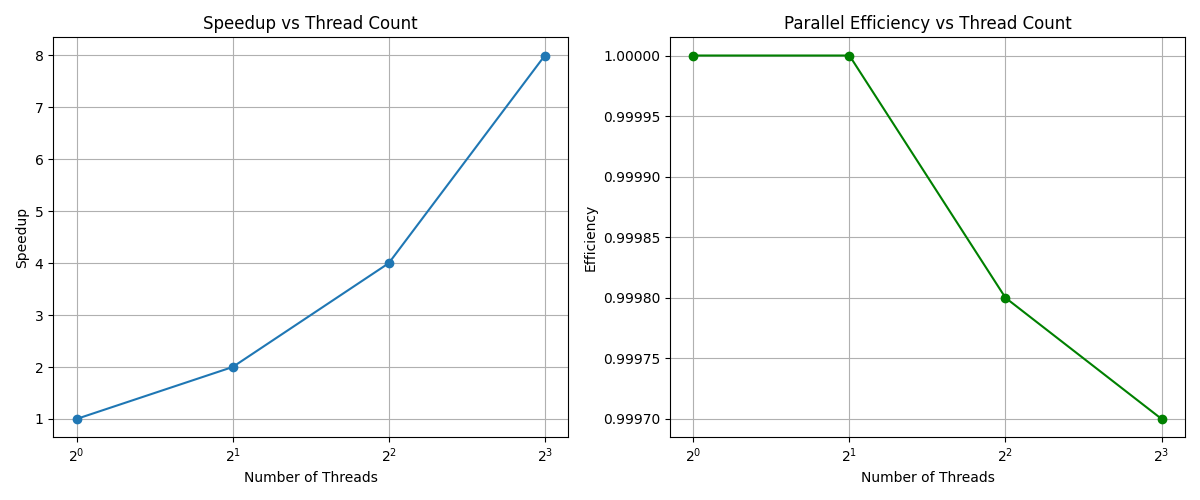
\includegraphics[width=0.9\textwidth]{./figures/Figure 5: updated_pi_scaling_plots.png}
\caption{Speedup and Parallel Efficiency for $\pi$ Approximation}
\label{fig:pi_scaling_plots}
\end{figure}


\newpage
\section{The Mandelbrot set using OpenMP \punkte{20}}


\newpage
\section{Bug hunt \punkte{15}}


\newpage
\section{Parallel histogram calculation using OpenMP \punkte{15}}


\newpage
\section{Parallel loop dependencies with OpenMP \punkte{15}}


\newpage
\section{Quality of the Report \punkte{15}}


\end{document}